\documentclass[svgnames]{beamer}

\usepackage{csspace-slides}

\title{Удивительная алгебра сравнения строк (часть 2)}

\author{\texorpdfstring{
    \Author{А. В. Тискин}{DPhil (Oxford),\ \ доцент МКН СПбГУ}
    \Author{Б. Золотов}{аспирант МКН СПбГУ}
}{}}


\begin{document}

\maketitle


\begin{frame}{\(\frac{3}{4}\)-local LCS}

\begin{center}
  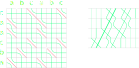
\includegraphics[width=9cm]{svg/34-local}
\end{center}

\end{frame}


\begin{frame}{Local LCS à la Sakai}
\end{frame}


\begin{frame}{Local LCS à la CGMW, T\color{red!28!white}{Z}}
\end{frame}


\begin{frame}{Динамическое выравнивание}

\begin{center}
  
\includegraphics[width=4cm]{svg/dynamic}
\end{center}

\end{frame}


\begin{frame}{Грассмановы перестановки}

\begin{center}
  \includegraphics[width=6.4cm]{img-fg/tP}
  
  \includegraphics[width=6.4cm]{img-fg/tP-FG}

  \includegraphics[width=6.4cm]{img-fg/tP-GF}
\end{center}

\end{frame}


\begin{frame}{Аффинное липкое умножение}

\begin{center}
  \includegraphics[width=4.5cm]{img-fg/PQ-base} \hspace{4mm}
  \includegraphics[width=4.5cm]{img-fg/PQ-GF3n} \vspace{2mm}

  \includegraphics[width=4.5cm]{img-fg/PQ-GF3n-untg} \hspace{4mm}
  \includegraphics[width=4.5cm]{img-fg/PQ-GF3n-z}  
\end{center}

\end{frame}


\begin{frame}{Периодическая задача LCS}
\end{frame}


\begin{frame}{Приближенный поиск подстрок}

\begin{block}{\vspace*{-3ex}}
  {\it Задача:} найти в тексте \(T\) подстроки, отличающиеся от шаблона \(P\) не более чем на редакционное расстояние \(k\).
\end{block} \vspace{4mm}

Ключевой шаг решения этой задачи~— {\it dynamic puzzle matching} строк с малым редакционным расстоянием:

\begin{block}{\vspace*{-3ex}}
  Дана эталонная строка \(U\) и семейство \(\mathcal F\).
  Известно, что \(\sum_{u \in \mathcal F} \delta (u, U) = O(k)\).
  Последовательность пар \((P_1, T_1) \ldots (P_Z, T_Z)\);\ \ 
  \(P_i, T_i \in \mathcal F\);\ \ пары могут в неё динамически
  вставляться и удаляться. Поддерживать вхождения
  \(P_1 \ldots P_Z\) в~\(T_1 \ldots T_Z\) с не более
  чем~\(k\) редакциями, быстро обновлять при вставке/удалении пары.
\end{block} \vspace{8mm}

\end{frame}


\begin{frame}{Dynamic puzzle maching}

Не отходим более чем на \(k\) от главной диагонали~— монжевы матрицы расстояний размером \(O(k)\).

\begin{center}
  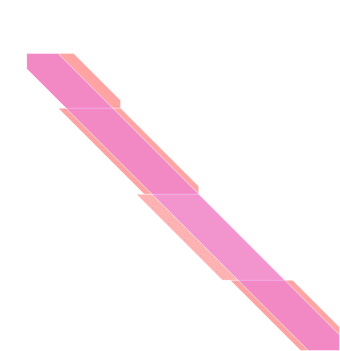
\includegraphics[width=4.8cm]{svg/wellnitz}
\end{center}

Построение: малое суммарное \(\delta\)~— применим динамическое выравнивание, чтобы построить матрицы расстояний для всех возможных пар.

\end{frame}


\end{document}
